%\section{Einführung}

\section{Modelling theory: Models in research}
%------------------------------------------------------------------------------
\begin{frame}{Models in research}

    % ----------------------------------------------
  \begin{columns}%[T,onlytextwidth]
  %\metroset{block=fill}
    \column{0.45\textwidth}
        \begin{quote}
        In den Wissenschaften werden Modelle aus den unterschiedlichsten Gründen zur Originalrepräsentation herangezogen.~\parencite[138]{stachowiak}
    \end{quote}
    \bigskip
    
    \begin{itemize}
        \item demonstration models
        \item experimental models
        \item theoretical models
        \item operative models
    \end{itemize}
    \bigskip
    
    \footnotesize
    
    For English summary of Stachowiak see: \protect\url{https://modelpractice.wordpress.com/2012/07/04/model-stachowiak/}
    % ----------------------------------------------

    \column{0.55\textwidth}

      \metroset{block=fill} % transparent

      \begin{alertblock}{All knowledge production happens in the context of models}
        \begin{quote}
Der Gewinn dieser Vorgehensweise \lbrack{}Modellierung\rbrack{} liegt
auf der Hand: Modellseitig gewonnene Einsichten und
Fertigkeiten lassen sich -- bei Erfülltsein gewisser
Transferierungskriterien -- auf das Original übertragen,
der Modellbildner gewinnt neue Kenntnisse über das
modellierte Original, er bekommt dieses besser als
bisher in den Griff, kann es auf neue Weise
zweckdienlich umgestalten oder als verbessertes
Hilfsmittel für neue Aktionen verwenden.~\parencite[140]{stachowiak}
        \end{quote}
      \end{alertblock}
  \end{columns}
\end{frame}

%------------------------------------------------------------------------------
\begin{frame}{Demonstration models}
  \begin{columns}%[T,onlytextwidth]
  \metroset{block=fill}
    \column{0.5\textwidth}
         \begin{quote}
        Als Demonstrationsmodelle werden sie zur
Veranschaulichung von (weniger anschaulichen oder
unanschaulichen) Zusammenhängen benutzt, \punkti.~\parencite[138]{stachowiak}
    \end{quote}\bigskip
    
    {\hfill 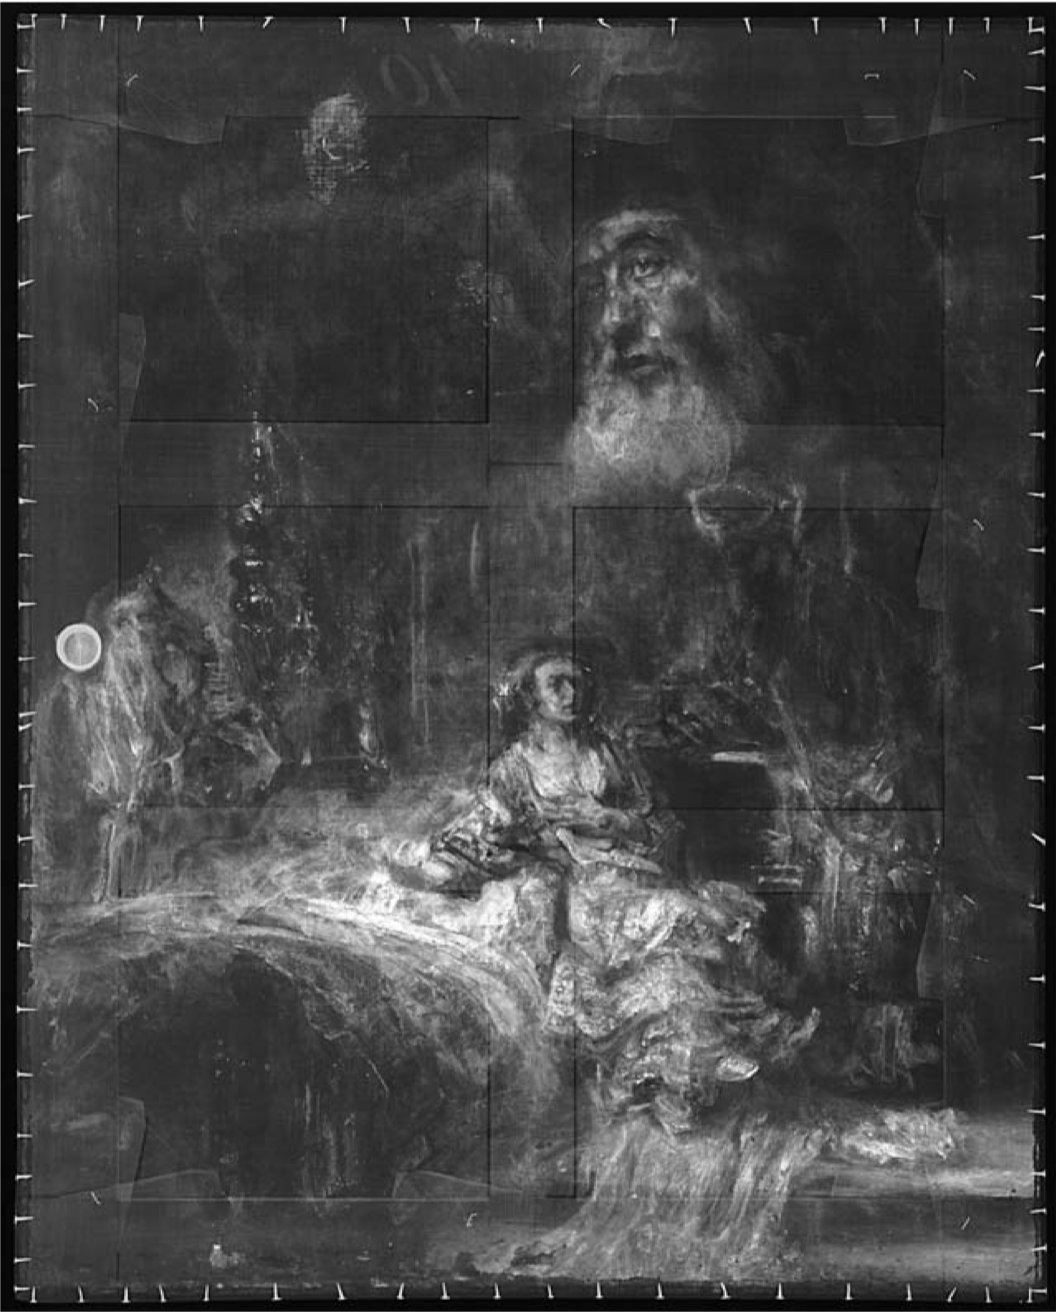
\includegraphics[width=0.5\textwidth]{img/demonstrationsmodell.png} \hfill}
    % ----------------------------------------------
    \column{0.5\textwidth}
    \begin{quote}
        So können etwa Veränderungen sichtbar gemacht
werden, die der Künstler während des Malens an einer
Komposition vorgenommen hat. Auch Manipulationen, die
von anderer Hand und zu einem späteren Zeitpunkt am
Original vorgenommen wurden, können auf diese Weise
„durchschaut“ werden.\\
{\scriptsize \href{https://web.archive.org/web/20140912212745/}{Link:} \href{http://www.arge-
kunstgeschichte.de/fileadmin/user\_upload/pdf/Der\_Blick\_durch\_die\_Bilder.pdf }{Der Blick durch die Bilder: Alte Meister geröntgt}, in: \protect\url{arge-kunstgeschichte.de}, S. 2.}
    \end{quote}

  \end{columns}
\end{frame}

%------------------------------------------------------------------------------

\begin{frame}[allowframebreaks]{Experimental models}
\metroset{block=fill}
\begin{quote}
„\punkti als Experimentalmodelle dienen sie der Ermittlung
oder Überprüfung von Hypothesen \punkti“~\parencite[139]{stachowiak}
\end{quote}
\begin{quote}
        Als Demonstrationsmodelle werden sie zur
Veranschaulichung von (weniger anschaulichen oder
unanschaulichen) Zusammenhängen benutzt, \punkti.~\parencite[138]{stachowiak}
\end{quote}\bigskip
    
    \begin{block}{Example}
    \begin{enumerate}\footnotesize
        \item \textbf{Hypothesis:} „The stronger the current, the lesser the pressure.“
        \item \textbf{Testing the hypothesis} using experiments
    \end{enumerate}
    \end{block}
    
    \framebreak
    
    \begin{columns}
    \column{0.45\textwidth}
    \begin{block}{}
        \href{https://youtu.be/K0aPuLn76H0}{Physics: Bernoulli effect}
    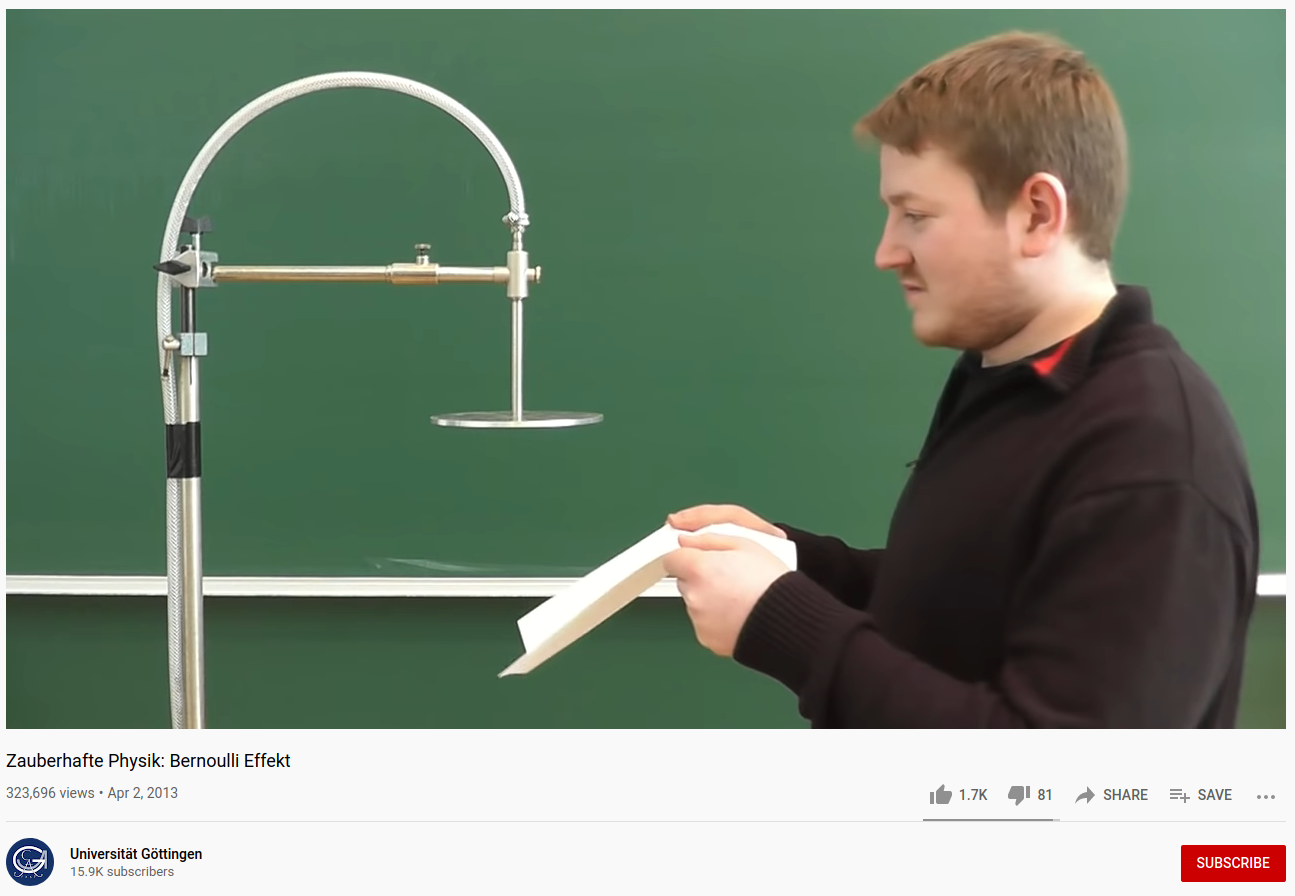
\includegraphics[width=\textwidth]{img/physik-bernoulli.png}
    \end{block}
    
    \column{0.45\textwidth}
    \begin{block}{}
        \href{https://www.youtube.com/watch?v=2vS4aPQI80M}{Recreating historical recipes}
    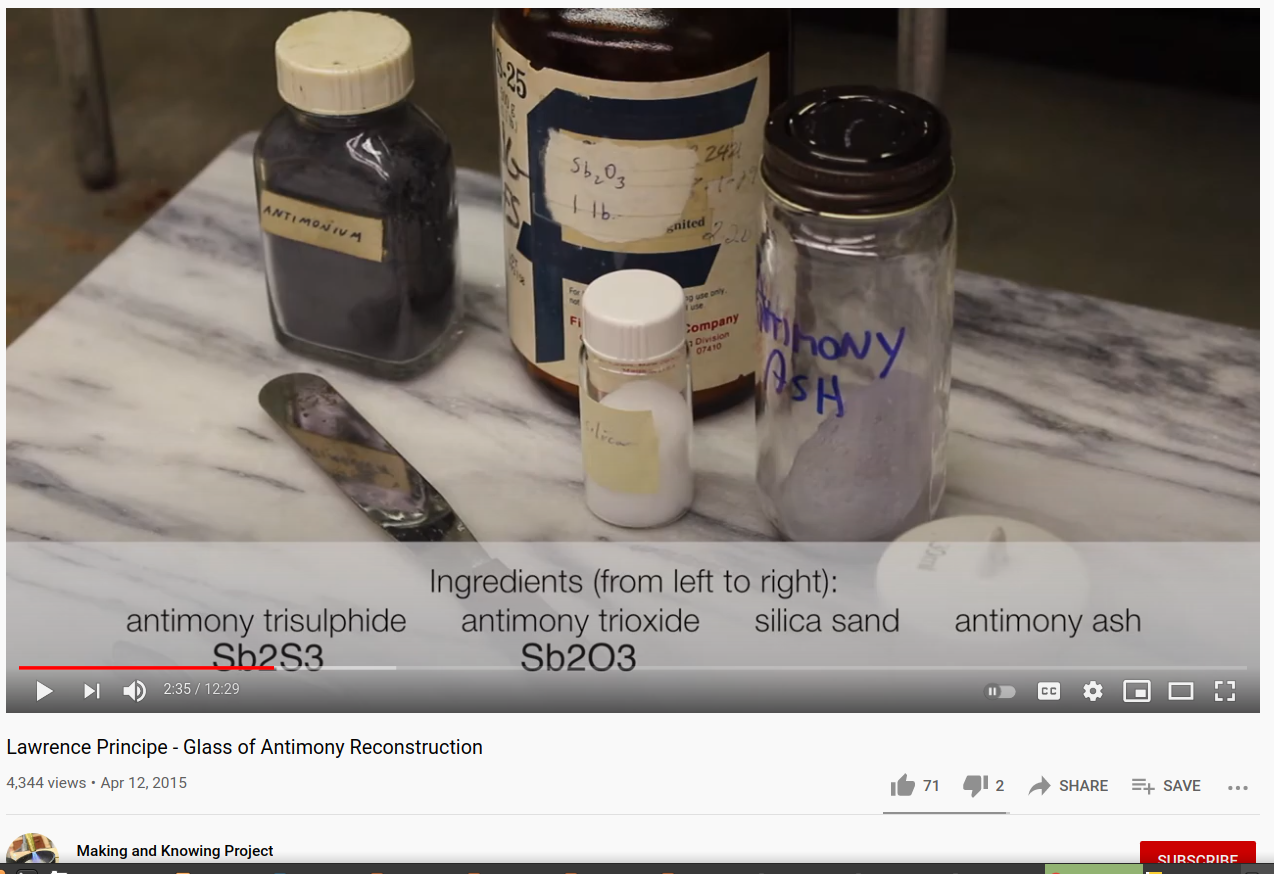
\includegraphics[width=\textwidth]{img/glass-of-antimony-experiment.png}
    
    \end{block}
    \end{columns}
    
\end{frame}

%------------------------------------------------------------------------------
\begin{frame}{Theoretical models}
  \begin{columns}%[T,onlytextwidth]
  \metroset{block=fill}
    \column{0.4\textwidth}
    \begin{block}{Stachowiak}
        \begin{quote}
            „\punkti als theoretische Modelle vermitteln sie in logisch bündiger Form Erkenntnisse über Sachverhalte,~\punkti“~\parencite[139]{stachowiak}.
        \end{quote}
    \end{block}

    % ----------------------------------------------
    \column{0.6\textwidth}
    \bigskip
    
    \begin{enumerate}
        \item \textbf{Rule:} All fish live in water.
        \item \textbf{Example:} Gold fish Hermann is a fish.
        \item \textbf{Result:} Hermann lives in water.
    \end{enumerate}
    \bigskip
    
    \begin{block}{Logic}
    $p \lor \neg p$
    \end{block}

  \end{columns}
\end{frame}

%------------------------------------------------------------------------------
\begin{frame}{Operative models}
  \begin{columns}%[T,onlytextwidth]
  \metroset{block=fill}
    \column{0.5\textwidth}
    \begin{quote} „Der wasserbauliche Modellversuch ist die beste
Methode, um Vorhersagen zu treffen, wie es in der
Natur aussieht, \punkti Die Ergebnisse der Untersuchungen sollen Aufschluss
darüber geben, ob das geplante Einlaufbauwerk
optimal dimensioniert ist und wann und wie die
Verschlüsse zu öffnen sind, um die gewünschte Wirkung
zu erzielen. \\
{\scriptsize \emph{Hochwasserschutz bei Kramsach im Modellversuch}, in: \protect\url{meinbezirk.at}. Stand: 04.02.2017.}
    \end{quote}
    % ----------------------------------------------
    \column{0.5\textwidth}
    \metroset{block=fill}
        \begin{block}{Stachowiak}
        \begin{quote}
            „\punkti und als operative Modelle möglicher Zielaußenwelten stellen sie ihren Benutzern Entscheidungs- und Planungshilfen zur Verfügung.“~\parencite[139]{stachowiak}
        \end{quote}
    \end{block}
    \metroset{block=fill}
      \begin{block}{}
      \href{https://www.youtube.com/watch?v=TbtdXpJvZiA\&t=78s}{Hochwasserschutz Radfeld}
      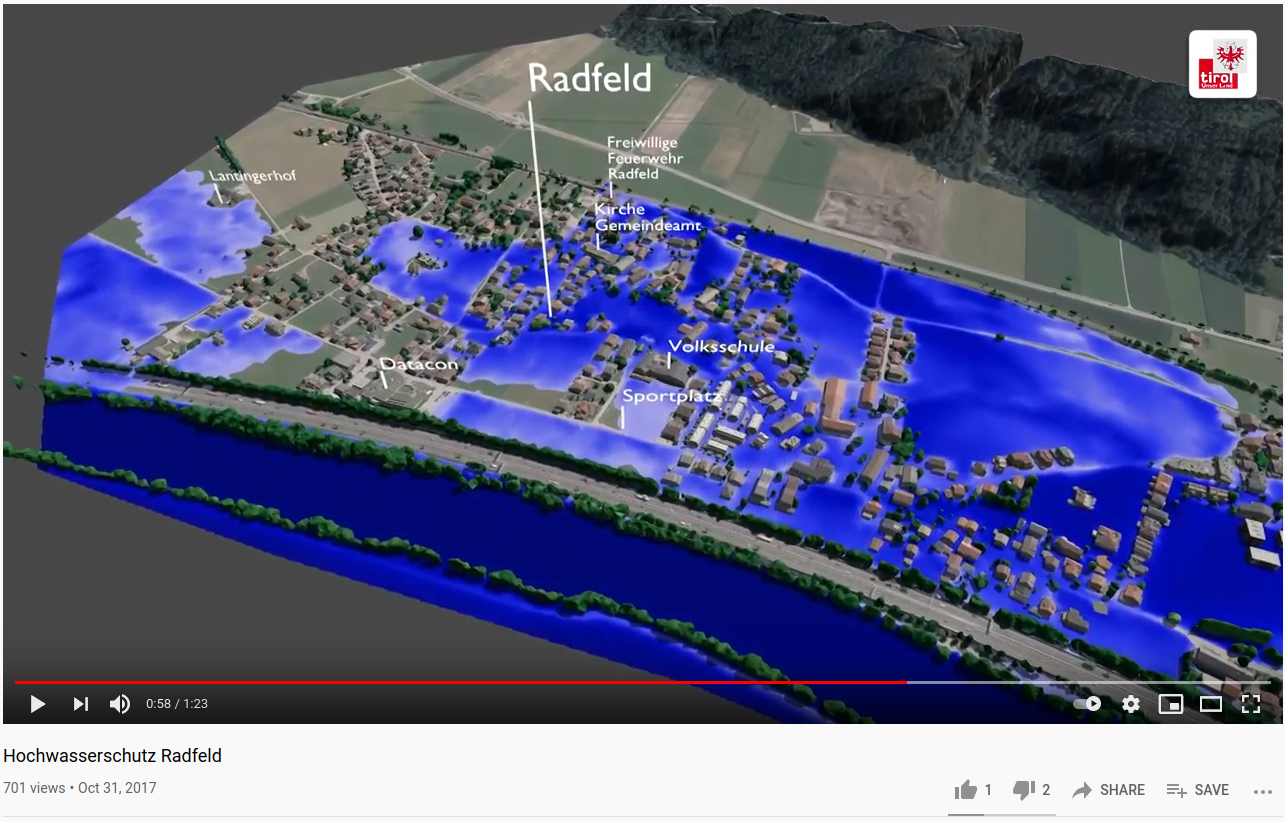
\includegraphics[width=0.95\textwidth]{img/radfeld-hochwasserschutz.png}
      \end{block}

  \end{columns}
\end{frame}

%------------------------------------------------------------------------------


%\begin{frame}[standout]    Homework and lecture\end{frame}
\subsection{Homework \& readings}

\begin{frame}{Homework: globe model}
\begin{itemize}
    \item the globe is a physical model of the world
    \item digital model = \href{https://www.google.at/maps/}{Google Maps}
    \begin{itemize}
        \item go on “Satellite“, zoom out.
        \item \href{https://earth.google.com}{Google Earth}
    \end{itemize}
    \item Which information or (abstract) knowledge is represented in those two models of the world?
    \item For which reasons or for what purpose can models (globe, Google Maps/Earth) be used to represent their original (the world)?
\end{itemize}

\metroset{block=fill}
\begin{alertblock}{Homework} \footnotesize
Take a globe or Google Maps/Earth, read chapters 2.1.3 of „Herbert Stachowiak: Allgemeine Modelltheorie“ (pdfs in the zip under "LEKTUERE", or in EN). If you can read it in German, please do so. 

Try to integrate what you have learned from reading Stachowiak.
Upload your solution (max. 1/2--1 page of text) to Moodle within the time period indicated.
The text should be readable, not bullet points. 
\end{alertblock}
\end{frame}

%------------------------------------------------------------------------------
\begin{frame}[standout]
    \alert{Reading} for next week: \\
    Stachowiak, all texts/PDFs (Nr. 02--04) \\
    \small (ca. 10 pages) 
\end{frame}
